% !TEX root = ../popl-paper.tex

In this section, we provide formal definitions of the asynchronous communication models we just presented 
informally based on an operational semantics and a notion of queuing network.

\paragraph{\bf Preliminaries}
For a finite set $S$, $\cardinalof{S}$ denotes the cardinal of $S$; $S^*$ denotes the set of finite words over $S$,
$w_1\cdot w_2$ denotes the concatenation of two words, $|w|$ denotes the length of $w$, and $\epsilon$ denotes the empty word. We assume some familiarity with non-deterministic
finite state automata,
and we write $\languageof{\A}$ for the language accepted
by the automaton $\A$. 
\etienne{Do we really need to talk about automata at that point?}

% For two sets $S$ and $I$,
% we write $\vect{b}$ (in bold) for an element of $S^I$,
% and $b_i$ for the $i$-th component of $\vect{b}$, so that
% $\vect{b}=(b_i)_{i\in I}$.

\paragraph{\bf Processes, messages, and actions}
We assume a finite set of \emph{processes} $\Procs=\{p,q,\ldots\}$ and a finite set of messages $\Msg=\{\msg,\ldots\}$. 
Each process may either (asynchronously) send a message to another one, or wait until it receives a message.
We therefore consider two kinds of actions. A \emph{send action} is of the form $\sact{p}{q}{\msg}$;
it is executed by process $p$ and sends message $\msg$ to process $q$.
The corresponding \emph{receive action} executed by $q$ is $\ract{p}{q}{\msg}$.
%
We write $\pqsAct{p}{q}$ to denote the set $\{\sact{p}{q}{\msg} \mid \msg \in \Msg\}$, and
$\pqrAct{p}{q}$ for the set $\{\ract{p}{q}{\msg} \mid \msg \in \Msg\}$.
Similarly, for $p \in \Procs$, we set
$\psAct{p} = \{\sact{p}{q}{\msg} \mid q \in \Procs 
% Etienne: shall we forbid processes to send messages to themselves?
%\setminus \{p\}
\}$ and $\msg \in \Msg\}$, etc.
Moreover, $\pAct{p} = \psAct{p} \cup \qrAct{p}$ denotes the set of all actions that are
executed by $p$.
Finally, $\Act = \bigcup_{p \in \Procs} \pAct{p}$
is the set of all the actions.

% A \emph{FIFO automaton} is basically a finite state machine equipped with 
% FIFO queues where transitions are labelled with either queuing or dequeuing actions. More precisely:
% \begin{definition}[FIFO automaton]
%   A \emph{FIFO automaton} is a tuple\footnote{
% Note that FIFO automata do not have accepting states, therefore they are
% not a special case of non-deterministic finite state automata, and
% there is not such a thing as \textquote{the language of a FIFO automaton}.
% }  
%   $\A=(L,\paylodSet,I,\actionSet,\delta,l_0)$
%   where
% (1) $L$ is a finite set of \emph{control states},
% (2) $\paylodSet$ is a finite set of \emph{messages},
% (3) $I$ is a finite set of \emph{buffer identifiers},
% (4) $\actionSet\subseteq I\times\{!,?\}\times\paylodSet$ is a finite set of \emph{actions},
% (5) $\delta\subseteq L\times \actionSet \times L$ is the \emph{transition relation}, and
% (6) $l_0\in L$ is the \emph{initial control state}.
% The \emph{size} $|\A|$ of $\A$ is $|L|+|\delta|$.
% \end{definition}

\paragraph{\bf Queuing networks}
We consider networks of processes formed by a bunch of FIFO queues that store the messages in transit. 
Formally, a \emph{queuing network} is a tuple $\anetwork=(\setofqueuidentifiers,\queuidofprocs)$ such that 
$\setofqueuidentifiers$ is a finite set of queue identifiers, and
$\queuidofprocs:\procSet\times\procSet\to \setofqueuidentifiers$ assigns a queue to each 
pair of processes. 
A queuing network $(\setofqueuidentifiers,\queuidofprocs)$ is $\pp$ if 
$\setofqueuidentifiers=\procSet\times\procSet$ and $\queuidofprocs$ is the identity.
The queuing network $(\setofqueuidentifiers,\queuidofprocs)$ is $\mb$ if 
$\setofqueuidentifiers=\procSet$ and $\queuidofprocs(p,q)=q$; it is called $\onen$ if
$\setofqueuidentifiers=\procSet$ and $\queuidofprocs(p,q)=p$. Finally, it is called
$\nn$ if $\setofqueuidentifiers=\{0\}$ and $\queuidofprocs(p,q)=0$ for all $p,q\in\procSet$.

\paragraph{\bf Configurations, executions, and operational semantics}
A \emph{configuration} of the queuing network $(\setofqueuidentifiers,\queuidofprocs)$ is 
a tuple $\aconf=(w_{\aqueueid})_{\aqueueid\in\setofqueuidentifiers}\in (\paylodSet^*)^{\setofqueuidentifiers}$,
where for each queue identifier $\aqueueid$, the queue content $w_{\aqueueid}$ is a finite sequence of messages.
The \emph{initial configuration} $\initconf$ is the one in which all queues are empty, i.e. 
$w_{\aqueueid}=\epsilon$ for all $\aqueueid\in\setofqueuidentifiers$.
A \emph{step} is a tuple $(\aconf,a,\aconf')$ (often written $\aconf\actionstep{a}\aconf'$)
where $\aconf=(w_{\aqueueid})_{\aqueueid\in\setofqueuidentifiers}$,
$\aconf'=(w_{\aqueueid}')_{\aqueueid\in\setofqueuidentifiers}$, 
$a$ is an action, and the following holds:
\begin{itemize}
  \item if $a=\sact{p}{q}{\msg}$, then $b'_{\aqueueid}=b_{\aqueueid}\cdot \msg$
  and $b_j'=b_j$ for all $j\in \setofqueuidentifiers\setminus\{\aqueueid\}$, 
  where $\aqueueid=\queuidofprocs(p,q)$.
  \item if $a=\ract{p}{q}{\msg}$, then $b_{\aqueueid}=\msg\cdot b'_{\aqueueid}$
  and $b_j'=b_j$ for all $j\in \setofqueuidentifiers\setminus\{\aqueueid\}$, 
  where $\aqueueid=\queuidofprocs(p,q)$.
\end{itemize}
An \emph{execution} of the queuing network $(\setofqueuidentifiers,\queuidofprocs)$
is a finite sequence of actions $e=a_1a_2\ldots a_n$ such that
$\initconf\actionstep{a_1}\actionstep{a_2}\ldots\actionstep{a_n}\aconf$ for some configuration $\aconf$.
The execution is $\pp$ (resp. $\mb$, $\onen$, $\nn$) if its queuing network is.

\begin{example}
The execution 
$$
\sact{p}{q}{m_1}\cdot\sact{q}{r}{m_2}\cdot\ract{q}{r}{m_2}\cdot\ract{p}{q}{m_1}
$$
is $\pp$, $\mb$, and $\onen$, but it is not $\nn$ (because $m_2$ is received before $m_1$). 
\end{example}

\begin{example}
    The execution 
    $$
    \sact{p}{q}{m_1}\cdot\sact{r}{q}{m_2}\cdot\ract{r}{q}{m_2}
    $$
    is $\pp$ and $\onen$, but it is neither $\mb$ nor $\nn$ (because $m_2$ "overtakes" $m_1$). Note that in the
    final configuration $m_1$ is still in the queue ($m_1$ is "unmatched"). 
\end{example}
    

Consider a network $\anetwork$ with two queue identifiers $\aqueueid_1$ and $\aqueueid_2$,
and let $\anetwork'$ be the network obtained by merging the two queues $\aqueueid_1$ and $\aqueueid_2$ in a 
same queue. Then $\anetwork'$ imposes more constraints than $\anetwork$ on the sequence of actions it admits, 
and any $\anetwork'$-execution also is an $\anetwork$-execution. From this observation, it follows that
the communication models we considered define the hierarchy of executions depicted in 
Fig.~\ref{fig:hierarchy-of-executions}; note that we did not cover the operational semantics of RSC,
causally ordered and fully asynchronous executions, and we refer to~\cite{DBLP:journals/fac/ChevrouHQ16}
for more details about how these other communication models fit in this hierarchy.

\begin{figure}
    % !TEX root = ../popl-paper.tex

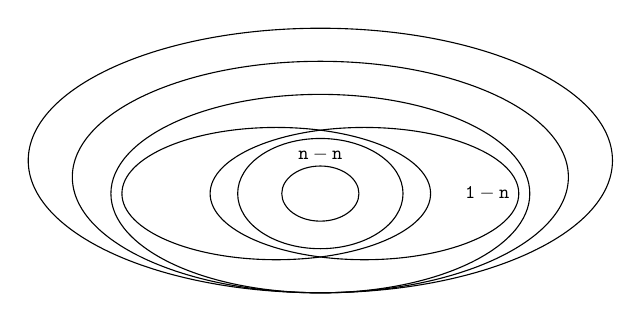
\begin{tikzpicture}[scale=0.7, every node/.style={transform shape}]
   % \draw (0,0) ellipse (5cm and 3cm);
    %\draw (0,0) ellipse (5cm and 3cm);
    %\draw (0,0) ellipse (5cm and 3cm);

\draw(0,0) ellipse (.7cm and .5cm); 
\node (r) at (0,0) {$\rsc$}; 
\draw(0,0) ellipse (1.5cm and 1cm); 
\node (nn) at (0,.7) {$\mathtt{n-n}$}; 

\draw(.8,0) ellipse (2.8cm and 1.2cm); 
\node[left] (n1) at (3.55,0) {$\mathtt{1-n}$}; 
\draw(-.8,0) ellipse (2.8cm and 1.2cm); 
\node[right] (1n) at (-3.5,0) {$\none$}; 

\draw(0,0) ellipse (3.8cm and 1.8cm); 
\node (nn) at (0,1.5) {$\co$}; 

\draw(0,.3) ellipse (4.5cm and 2.1cm); 
\node (nn) at (0,2) {$\oneone$}; 

\draw(0,.6) ellipse (5.3cm and 2.4cm); 
\node (nn) at (0,2.6) {$\asy$}; 

\end{tikzpicture} 

% \begin{tikzpicture}[inclusion/.style={right hook->, thick}]
%     \node (RSC)    at (-1.7,0) {\begin{tabular}{c}synchronous \\ (RSC)\end{tabular}};
%     \node (FIFOnn) at (1,0)  {\begin{tabular}{c}FIFO \\ n-n\end{tabular}}; 
%     \node (FIFO1n) at (3.2,1.5)  {\begin{tabular}{c}FIFO 1-n\end{tabular}};
%     \node (mb)     at (3.2,-1.5) {\begin{tabular}{c}FIFO n-1\\ (mailbox)\end{tabular}};
%     \node (co)     at (5.8,0)  {\begin{tabular}{c}causally\\ ordered\end{tabular}};
%     \node (p2p)    at (8,0) {\begin{tabular}{c}FIFO 1-1\\ (p2p)\end{tabular}};
%     \node (async)  at (10.4,0) {\begin{tabular}{c}asyn-\\ chronous\end{tabular}};
%     \draw[inclusion] (RSC) to (FIFOnn);
%     \draw[inclusion] (FIFOnn.north east) to (FIFO1n.west);
%     \draw[inclusion] (FIFOnn.south east) to (mb.west);
%     \draw[inclusion] (FIFO1n.east) to (co.north west);
%     \draw[inclusion] (mb.east) to (co.south west);
%     \draw[inclusion] (co) to (p2p);
%     \draw[inclusion] (p2p) to (async);
% \end{tikzpicture}
    \caption{\label{fig:hierarchy-of-executions} The hierarchy of communication models based on their sets of
    executions (taken from~\cite{DBLP:journals/fac/ChevrouHQ16})}
\end{figure}